\documentclass[
ngerman,
twoside,
pdfa=false,
ruledheaders=section,%Ebene bis zu der die Überschriften mit Linien abgetrennt werden, vgl. DEMO-TUDaPub
class=report,% Basisdokumentenklasse. Wählt die Korrespondierende KOMA-Script Klasse
thesis={type=sta},% Dokumententyp Thesis, für Dissertationen siehe die Demo-Datei DEMO-TUDaPhd
accentcolor=TUDa-2c,% Auswahl der Akzentfarbe
custommargins=false,% Ränder werden mithilfe von typearea automatisch berechnet
marginpar=false,% Kopfzeile und Fußzeile erstrecken sich nicht über die Randnotizspalte
%BCOR=5mm,%Bindekorrektur, falls notwendig
parskip=half-,%Absatzkennzeichnung durch Abstand vgl. KOMA-Sript
fontsize=11pt,%Basisschriftgröße laut Corporate Design ist mit 9pt häufig zu klein
%	logofile=tuda_logo.pdf, %Falls die Logo Dateien nicht installiert sind
]{tudapub}

%%%%%%%%%%%%%%%%%%%%%%%%%%%%
% Download des TU-Logos
%%%%%%%%%%%%%%%%%%%%%%%%%%%%
% https://download.hrz.tu-darmstadt.de/protected/CE/TUDa_LaTeX/tuda_logo.pdf
% Der Pfad zum Logo kann als "logofile" angegeben werden.

%%%%%%%%%%%%%%%%%%%
% Sprachanpassung & Verbesserte Trennregeln
%%%%%%%%%%%%%%%%%%%
\usepackage[english, main=ngerman]{babel}
\usepackage[autostyle]{csquotes}% Anführungszeichen vereinfacht
\usepackage{microtype}

%%%%%%%%%%%%%%%%%%%
% Literaturverzeichnis
%%%%%%%%%%%%%%%%%%%
\usepackage{biblatex}   % Literaturverzeichnis
\addbibresource{HausarbeitBib.bib}

%%%%%%%%%%%%%%%%%%%
% Paketvorschläge Tabellen
%%%%%%%%%%%%%%%%%%%
%\usepackage{array}     % Basispaket für Tabellenkonfiguration, wird von den folgenden automatisch geladen
\usepackage{tabularx}   % Tabellen, die sich automatisch der Breite anpassen
%\usepackage{longtable} % Mehrseitige Tabellen
%\usepackage{xltabular} % Mehrseitige Tabellen mit anpassarer Breite
\usepackage{booktabs}   % Verbesserte Möglichkeiten für Tabellenlayout über horizontale Linien

%%%%%%%%%%%%%%%%%%%
% Paketvorschläge Mathematik
%%%%%%%%%%%%%%%%%%%
\usepackage{mathtools} % erweiterte Fassung von amsmath
\usepackage{amssymb}   % erweiterter Zeichensatz
\usepackage[decimalsymbol=comma]{siunitx}   % Einheiten
\usepackage{amsmath}


%%%%%%%%%%%%%%%%%
% Eigenen Pakete Gruppe01
%%%%%%%%%%%%%%%%%%%%
%\usepackage[utf8]{inputenc}
%\usepackage[ngerman]{babel}
\usepackage{hyperref}
\usepackage{graphicx}
\usepackage{subcaption}
\usepackage{listings}
\usepackage[framed, numbered]{matlab-prettifier}
%\usepackage[style=numeric]{biblatex}
%\usepackage{amsthm}
%\usepackage[squaren]{SIunits}
\usepackage{enumitem}
\usepackage{tikz}
\usepackage{pgfplots}
\usepackage{pgfplotstable}
%\usepackage{booktabs}
\pgfplotsset{compat=1.12}
\usepackage{dsfont}

%%%%%%%%%%%%%%%%%%%
% verschiedene Nummerierung für Abbildungen und Formeln
%%%%%%%%%%%%%%%%%%%
\usepackage{chngcntr}
\counterwithout{equation}{chapter}


%%%%%%%%%%%%%%%%%%%
% Pseudocode
%%%%%%%%%%%%%%%%%%%
\usepackage[linesnumbered,lined,boxruled]{algorithm2e} % Package für Pseudocode

%%%%%%%%%%%%%%%%%%%
% Plotting und Grafik
%%%%%%%%%%%%%%%%%%%
\usepackage{tuda-pgfplots} % Package für Plotting with TUDa mods

%%%%%%%%%%%%%%%%%%%
% Sonstiges
%%%%%%%%%%%%%%%%%%%
\usepackage{blindtext} % Package für Blindtext

\begin{document}
	\title{Ausarbeitung Übung 5}
	%\subtitle{Ein Untertitel, wenn nötig}
	\author[D. Schiller, C. Kramer, S.Arnold, T. Lingenberg]{Dominik Schiller \and Constanze Kramer \and Simon Arnold \and Tobias Lingenberg} %optionales Argument ist die Signatur,
	%\reviewer{Gutachter 1 \and Gutachterin 2} %Gutachten
	
	%Diese Felder werden untereinander auf der Titelseite platziert.
	\department{} % Das Kürzel wird automatisch ersetzt und als Studienfach gewählt, siehe Liste der Kürzel im Dokument.

	
	\date{\today}
	%\examdate{\today}
	
	%	\tuprints{urn=1234,printid=12345}
	%	\dedication{Für alle, die \TeX{} nutzen.}
	
	\maketitle
	\pagenumbering{gobble} % Seitenzahlen angezeigt, startet ab dem Inhaltsverzeichnis
	
	
	%\affidavit
	%\AffidavitSignature
	%\AffidavitSignature
	
	
	%%%%%%%%%%%%%%%%%%%
	%Abstract / Kurzzusammenfassung
	%%%%%%%%%%%%%%%%%%%
	%\include{chapters/zusammenfassung}
	
	%%%%%%%%%%%%%%%%%%%
	%Inhaltsverzeichnis 
	%%%%%%%%%%%%%%%%%%%
	\cleardoublepage
	\tableofcontents % Erstellte ein Inhaltsverzeichnis
	
	%\cleardoublepage
	\pagenumbering{arabic} % Seitenzahlen angezeigt, startet ab dem Inhaltsverzeichnis
	\setcounter{page}{1} % Setzt den Seitenzahlenzähler auf 1
	
	%%%%%%%%%%%%%%%%%%%%%%%%%%%%%%%%%%%%%%%%%%%%%%%%%%%%%%%%%%%%%%%%%%%%%%%%%%%%%%%%%%%%%%%%%%%%%%%%%%
	
	% INHALT, am Besten ausgelagert in eigene Files/Kapitel und dann mit \include{Unterordner/Filename} eingefügt, sorgt für bessere Übersichtlichkeit und Fehlersuche. Einzelne Dateien sind aktuell im Ordner Sections abgelegt. 
	%%%%%%%%%%%%%%%%%%Einleitung%%%%%%%%%%%%%%%%%
	%\chapter{Einleitung}\label{sec:intro}
Diese Arbeit beschäftigt sich mit dem Übungsblatt 9 des Faches \glqq Einführung in die numerische Berechnung elektromagnetischer Felder\grqq{}.
Zunächst wird der primale Divergenz und Rotationsoperator in Octave implementiert und berechnet. Anschließend wird eine Materialmatrix berechnet. Abschließend wird das Magnetfeld von zwei stromdruchflossenen Leitern in Octave simuliert. 
	%%%%%%%%%%%%%%%%%%Haupteil%%%%%%%%%%%%%%%%%%%
	\include{chapters/ag5_2}
	\section{Homogener Kugelkondensator}
Wie in den vorherigen Aufgaben und Ausarbeitungen gezeigt, lassen sich mit Hilfe von FEMM sehr gute Simulationen von Plattenkondensatoren erzeugen. Aber auch Kugelkondensatoren lassen sich mit FEMM simulieren und berechnen. \\
Die Methode \texttt{spherecapacity.m}, die im Anhang zu finden ist, nimmt die zwei Parameter $R_1$, der den Innenradius beschreibt und $\varepsilon_r$, das die relative Permittivität des Dielektrikums darstellt, entgegen. Aus der Aufgabenstellung geht hervor, dass für den zweiten zur Berechnung der Kapazität benötigten Parameter $R_2 = R_1 + \SI{7}{\centi\meter}$ gilt. $R_2$ ist der Außenradius des Kugelkondensators. Optional könnte man die Methode auch so schreiben, dass $R_2$ übergeben werden kann.\\
Im Vergleich zu den bisherigen Simulationen in FEMM haben wir nun kein planares Problem mehr, sondern ein achsensymmetrisches. In der Problemdefinition (Zeile 6) wird deshalb ein \texttt{'axi'} übergeben. Damit wird bestimmt, dass sich die erzeugte Fläche in Abbildung \ref{fig:KK} nicht in die Tiefe entwickelt, sondern um die z-Achse gedreht wird. Dadurch erhält man eine 3-Dimensionale Kugel, die FEMM zwar nicht darstellen, aber berechnen kann.\\ \\
Zunächst werden zwei Halbkreise erzeugt (Zeile 12-26), zwischen diesen beiden Halbkreisen liegt eine Spannungsdifferenz von \SI{1}{\volt} an. Des Weiteren werden zwei Blocklabel erstellt (Zeile 28 und 31), das erste Label liegt zwischen den beiden Halbkreisen und beinhalten die Informationen über die relative Permittivität des Dielektrikums. Mit dem zweiten Label wird sichergestellt, dass nur die von den beiden Halbkreisen und deren Verbindungslinien eingeschlossene Fläche bei der Berechnung berücksichtigt wird. Hierzu wird dem Label die Property \texttt{'<No Mesh>'} übergeben. Schließlich werden die Verbindungslinien zwischen den Halbkreisen erstellt(Zeile 38 und 39), um eine abgeschlossene Fläche zu erzeugen. \\ \\
\begin{figure}[h]
	\centering
	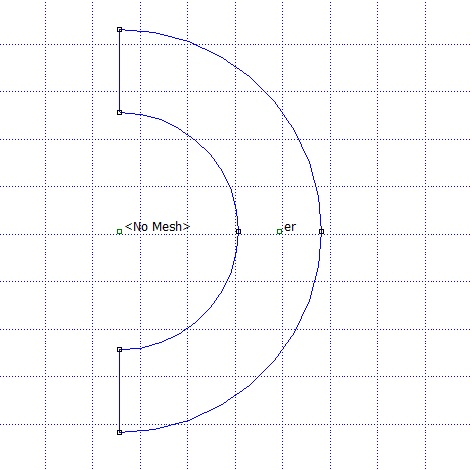
\includegraphics[width=.45\textwidth]{data/Kugelkondensator}
	\caption{Ein mit Hilfe der Routine \texttt{spherecapacity.m} erzeugter Kugelkondensator mit $R_1 = \SI{7}{\centi\meter}$ }
	\label{fig:KK}
\end{figure}

Mit 
\begin{equation}
	C = 4\pi\varepsilon_0\varepsilon_r\frac{R_2R_1}{R_2-R_1}
	\label{eq:Kapa}	
\end{equation}
lässt sich die Kapazität eines homogenen Kugelkondensators berechnen.
Um den Einfluss der Radien auf die Kapazität zu untersuchen, wurden der Methode \texttt{spherecapacity.m} 100 verschiedene Radien $R_1 \in \mathbb{N}, R_1 \in [1,100]$, mit der Einheit \si{\centi\meter} übergeben. Für den Radius $R_2$ gilt weiterhin
\begin{equation}
	R_2 = R_1 + \SI{7}{\centi\meter}.
	\label{eq:R2}
\end{equation}
Die berechneten Kapazitätswerte sind in Abbildung \ref{fig:Kapa} graphisch dargestellt. Die Formel 
\begin{equation}
	C = 4\pi\varepsilon_0\varepsilon_r\frac{(R_1+\SI{7}{\centi\meter})R_1}{R_1+\SI{7}{\centi\meter-R_1}}
\end{equation}
ergibt sich indem man (\ref{eq:R2}) in (\ref{eq:Kapa}) einsetzt. Durch weiteres vereinfachen folgt, dass die Kapazität
\begin{equation}
	C = 4\pi\varepsilon_0\varepsilon_r\frac{R_1^2+\SI{7}{\centi\meter}}{\SI{7}{\centi\meter}}
\end{equation}
quadratisch von $R_1$ abhängt, dies erklärt den quadratischen Verlauf der Kapazität (Abbildung \ref{fig:KK}) des Kugelkondensators mit steigendem Innenradius.

\begin{figure}
	\centering
	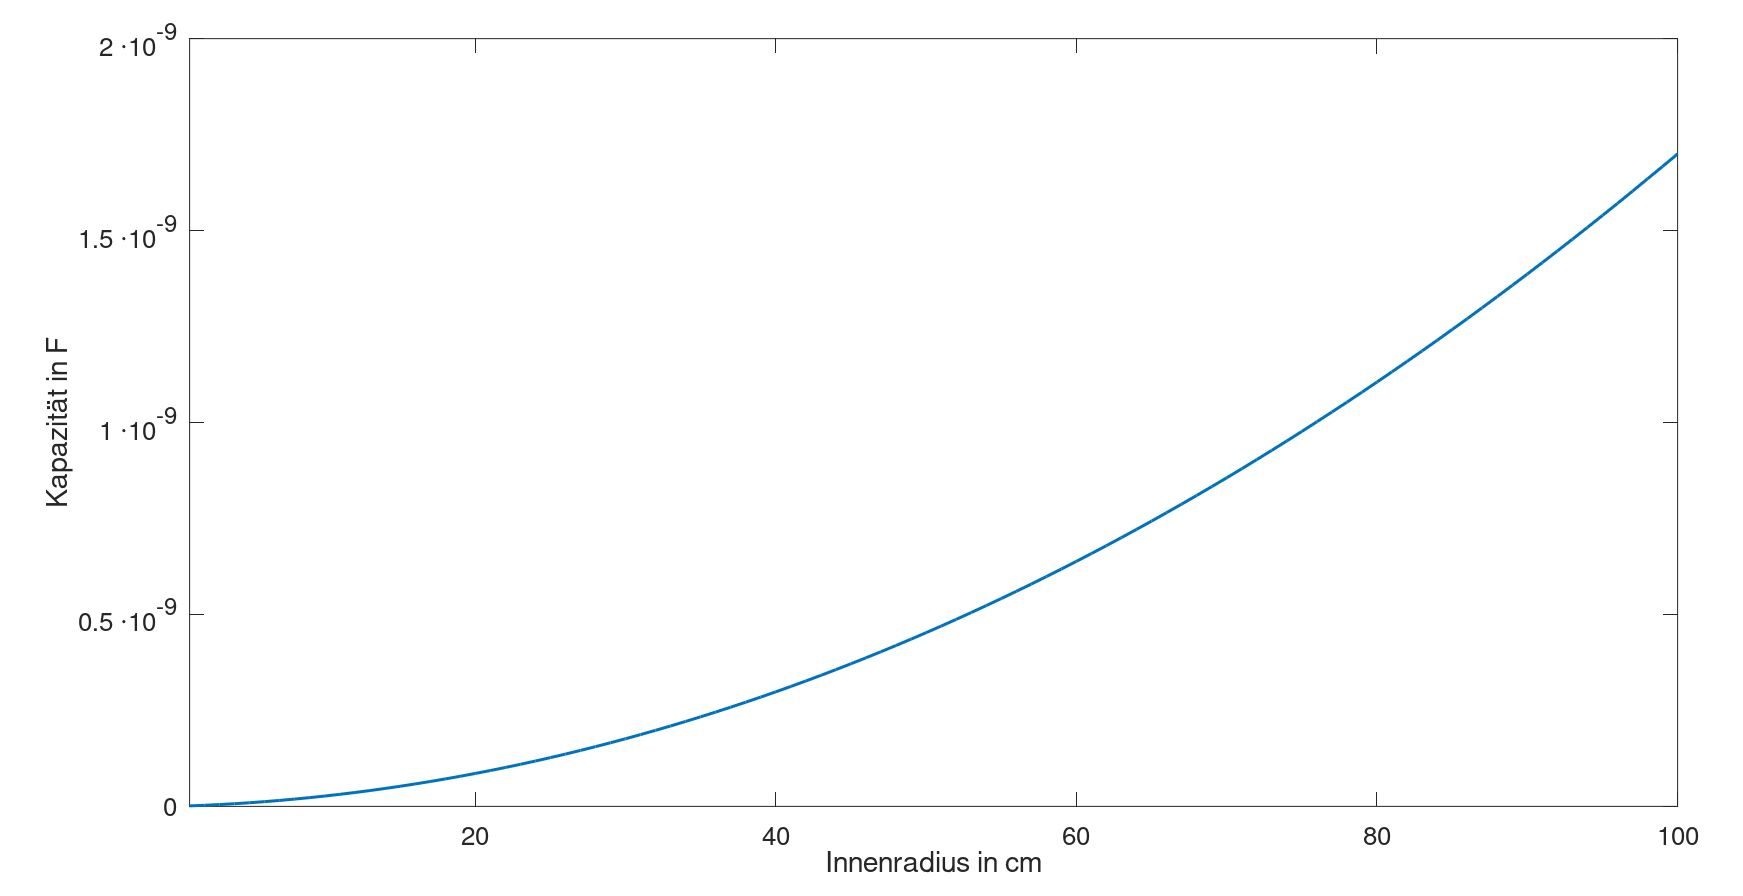
\includegraphics[width=\textwidth]{data/Kugelkapa}
	\caption{Verlauf der Kapazität mit steigendem Radius $R_1$ und $R_2 = R_1 + \SI{7}{\centi\meter}$}
	\label{fig:Kapa}
\end{figure}
\newpage
Unter der Voraussetzung, dass $(R_2+R_1) = \SI{15}{\centi\meter}$ gilt, beträgt der Innenradius $R_1 = \SI{4}{\centi\meter}$ und der Außenradius $R_2 = \SI{11}{\centi\meter}$. Analytisch lässt sich mit (\ref{eq:Kapa}) eine Kapazität $C_{\mathrm{ana}} = \SI{6,994}{\pico\farad}$ berechnen, FEMM berechnet eine Kapazität $C_{\mathrm{num}} = \SI{6,986}{\pico\farad}$. \\ \\
Der relative Fehler
\begin{equation}
	\mathrm{err :=} \frac{|C_{\mathrm{ana}}-C_{\mathrm{num}}|}{|C_{\mathrm{ana}}|}
	\label{eq:err}
\end{equation}
ergibt sich mit den vorher berechneten Werten $C_{\mathrm{ana}}$ und $C_{\mathrm{num}}$ zu $1.1 \cdot 10^{-3}$, liegt also im niedrigen Promillebereich. Die durch FEMM berechnete Annäherung ist sehr exakt.
	Bestimmt werden soll nun, für welche Werte $R_1$ und $R_2$ die Kapazität den Wert
$C = \SI{5}{\pico\farad}$ an nimmt.

\subsection*{Analytische Betrachtung}
Mithilfe der Formel \ref{eq:Kapa} gelten folgende Zusammenhänge:

\begin{equation}
\SI{5}{\pico\farad} = 4\pi\varepsilon_0\varepsilon_r\frac{R_2R_1}{R_2-R_1} \text{, sowie } 
R_2 = R_1 + \SI{7}{\centi\meter}
\end{equation}

Einsetzen der zweiten Formel liefert eine quadratische Gleichung für $R_1$

\begin{equation}
\SI{5}{\pico\farad} = 4\pi\varepsilon_0\varepsilon_r\frac{R_1(R_1+\SI{7}{\centi\meter})}{\SI{7}{\centi\meter}}
\end{equation}

Für die man Folgendes Ergebnis erhält:

\begin{equation}
R_1 = \SI{-7/2}{\centi\meter} \pm \sqrt{\left(\SI{7/2}{\centi\meter}\right)^2 + \dfrac{\SI{7}{\centi\meter} \cdot \SI{5}{\pico\farad}}{4\pi\varepsilon_0\varepsilon_r}}
\end{equation}

Dabei ist nur das Ergebnis $R_1 = \SI{3.1111}{\centi\meter}$ positiv und in diesem Zusammenhang sinnvoll.

\subsection*{Numerische Betrachtung}

Um das Problem numerisch zu untersuchen, wurde zunächst das Bisektionsverfahren (siehe Listing \ref{list:bisektion}) in Octave implementiert. Dieses erlaubt durch wiederholte Intervallhalbierung Nullstellen komplizierter Funktionen näherungsweise zu bestimmen. Die Wahl der Startpunkte ist hierbei für die Konvergenz entscheidend. Voraussetzung ist, dass beide Funktionswerte zu den Startwerten $a$ und $b$ unterschiedliche Vorzeichen haben und die gesuchte Nullstelle auch in diesem Intervall liegt. Durch vorherige Abschätzungen wurden die Startwerte $a=1$ und $b=10$ für den Methodenaufruf gewählt (siehe Listing \ref{list:ag5.3d}).

Die numerische Berechnung ergab die Lösung $R_1 = \SI{3.1130}{\centi\meter}$. Das entspricht einer Abweichung von $\SI{19}{\micro\meter}$ zu dem zuvor berechneten Wert.

\subsection*{Fehlerbetrachtung}

Die analytische Lösung ist exakt. Folglich entstehen auf numerischem Weg Ungenauigkeiten, die aus Rundungsfehlern resultieren. Besonders das Rechnen mit sehr großen und sehr kleinen Zahlen gleichzeitig kann unter Umständen am Computer zu Problemen führen, wenn Basisoperationen mit nicht ausreichender Stellenanzahl durchgeführt werden. Fehleranfällig kann jedoch auch schon die Simulation in FEMM sein. Da dort das Problem nur durch ein diskretes, also nicht exaktes, Modell simuliert wird.

Jedoch lässt sich auch in der Realität ein Versuchsaufbau nicht Fehlerfrei gestalten. So können dort Störeffekte durch bspw. externe Magnetfelder oder geringfügig inhomogene Dielektrika auftreten. Zudem ist auch einfach die Messgenauigkeit der Instrumente beschränkt. 
	
	%%%%%%%%%%%%%%%%%%Fazit%%%%%%%%%%%%%%%%%%%%%%
	%\chapter{Fazit}\label{sec:fazit}
%\addcontentsline{toc}{section}{Fazit}
Die erste Aufgabe ergab, dass sich die beiden Leiter des Koaxialkabels wie die Platten eines Plattenkondensators verhalten. Darüber hinaus ergibt sich, dass man durch Anfügen von weiteren Segmenten an die Schaltung eine Verkleinerung der Schwingfrequenz bewirkt.
Differentialgleichungen können häufig, wie sich in Aufgabe zwei zeigt, leichter im Frequenzbereich als im Zeitbereich gelöst werden. Die durch Lösen der Differentialgleichung analytisch berechneten Ergebnisse für Zeit- und Frequenzverhalten stimmen dabei mit der numerischen Simulation durch LTSpice überein.
Die Ergebnisse der dritten Aufgabe ergeben, dass sich die Feldlinien eines Kondensators in einem Simulationskäfig nicht nur senkrecht zu den Platten bewegen, sondern dass sich auch Randeffekte an den Enden der Kondensatorplatten ausbilden. Untersucht man unterschiedliche Randbedingungen zeigt sich, dass diese sowohl den Kapazitätswert des Kondensators, als auch die elektrischen Feldlinien beeinträchtigen. Die Wahl der Simulationsrandbedingungen kann also nicht willkürlich erfolgen.
	%%%%%%%%%%%%%%%%%%Anhang%%%%%%%%%%%%%%%%%%%%%
	\chapter{Anhang}\label{sec:anhang}
\lstset{ % Octave Settings
	language=Octave,
	extendedchars=true,
	basicstyle=\footnotesize,
	numbers=left,
	numberstyle=\tiny\color{gray},
	stepnumber=1,
	numbersep=10pt,
	showspaces=false,
	showstringspaces=false,
	tabsize=2,
	breaklines=true,
	frame=single,
	morecomment = [l][\itshape\color{blue}]{\%},
	captionpos=b,
	title=\lstname
}


\lstinputlisting{data/SIS.m}
\lstinputlisting{data/SkriptAg8_2.m}
\lstinputlisting{data/SkriptAg8_3d.m}



	%%%%%%%%%%%%%%%%%%%%%%%%%%%%%%%%%%%%%%%%%%%%%%%%%%%%%%%%%%%%%%%%%%%%%%%%%%%%%%%%%%%%%%%%%%%%%%%%%%
	
	%%%%%%%%%%%%%%%%%%%
	%Abbildungs- und Tabellenverzeichnis
	%%%%%%%%%%%%%%%%%%%
	\listoffigures % Abbildungsverzeichnis (captions in den Figuren werden als Referenz genommen)
	%\listoftables % Verzeichnis der Tabellen (captions in den Tabellen werden als Referenz genommen)
	
	%%%%%%%%%%%%%%%%%%%
	%Literaturverzeichnis an dieser Stelle
	%%%%%%%%%%%%%%%%%%%
	
	
\end{document}
